% !TEX program = xelatex
\documentclass[tikz, crop, border = {2pt 2pt 2pt 2pt}]{standalone}

\usepackage{concmath-otf}
\usetikzlibrary{calc, angles, quotes, patterns}
\usetikzlibrary{decorations.pathreplacing, decorations.pathmorphing, calligraphy}

\begin{document}
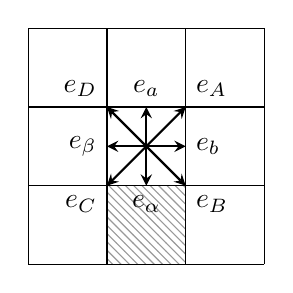
\begin{tikzpicture}
	\newcommand{\e}{\pmb{\symrm{e}}}
	\draw (-1, 2) grid (2, -1);
	\filldraw[pattern = north west lines, pattern color = black!40] (0, 0) rectangle (1, -1);
	\coordinate (A) at (0.5, 0.5);
	\draw (0, 0) rectangle (1, 1);
	\draw[-stealth, thick] (A) -- ++ (1/2, 0)    node[at end, right]{$\e_b$};
	\draw[-stealth, thick] (A) -- ++ (0, 1/2)    node[at end, above]{$\e_a$};
	\draw[-stealth, thick] (A) -- ++ (-1/2, 0)   node[at end, left]{$\e_{\beta}$};
	\draw[-stealth, thick] (A) -- ++ (0, -1/2)   node[at end, below]{$\e_{\alpha}$};
	\draw[-stealth, thick] (A) -- ++ (1/2, 1/2)  node[at end, above right]{$\e_A$};
	\draw[-stealth, thick] (A) -- ++ (-1/2, 1/2) node[at end, above left]{$\e_D$};
	\draw[-stealth, thick] (A) -- ++ (-1/2, -1/2)node[at end, below left]{$\e_C$};
	\draw[-stealth, thick] (A) -- ++ (1/2, -1/2) node[at end, below right]{$\e_B$};
\end{tikzpicture}
\end{document}
